\documentclass[11pt,a4paper]{article}
\usepackage{float}
\usepackage[utf8]{inputenc}
\usepackage[left=2cm,right=2cm,text={18cm,24cm},top=2cm]{geometry}
\usepackage[czech]{babel}
\usepackage{graphicx}
\usepackage{verbatim}
\usepackage{fancyvrb}
\usepackage{svg}
\usepackage{biblatex}
\usepackage{hyperref}
\usepackage{tabto}
\usepackage{rotating}
\usepackage{listings}

\renewcommand{\familydefault}{\sfdefault}

\begin{document}

\begin{center}
    \includegraphics[scale=0.3]{include/fit.pdf} \\  
    \textbf{\Large{ISS projekt 2022 \\
    Protokol řešení}} \\
    Matyáš Strelec (xstrel03) \\
    \today
\end{center}

Celý zdrojový kód řešení projektu je v souboru \verb|reseni.ipynb| s příslušnými komentáři ke všem částem a jednotlivým kusům kódu.

\section{Základy}

V první části načítám 0.5 sekundy každého tónu, od začátku posunuté o 0.25 sekund.

Pro zobrazení 3 period je potřeba spočítat délka 1 periody vzorcem $\frac{F_s}{f}$, kde $F_s$ je vzorkovací frekvence a $f$ je frekvence tónu. Přepočet vzorků na milisekundy je pomocí vzorce $\frac{1}{F_s}*1000$.

Pro zobrazení spektra tónu je použita funkce \verb|np.fft()|. Pro délku spektra 24000 Hz je potřeba 0.5sekundový tón doplnit nulami na její dvojnásobek. Je zobrazena absolutní hodnota spektra v log PSD.

\begin{figure}[H]
    \begin{center}
        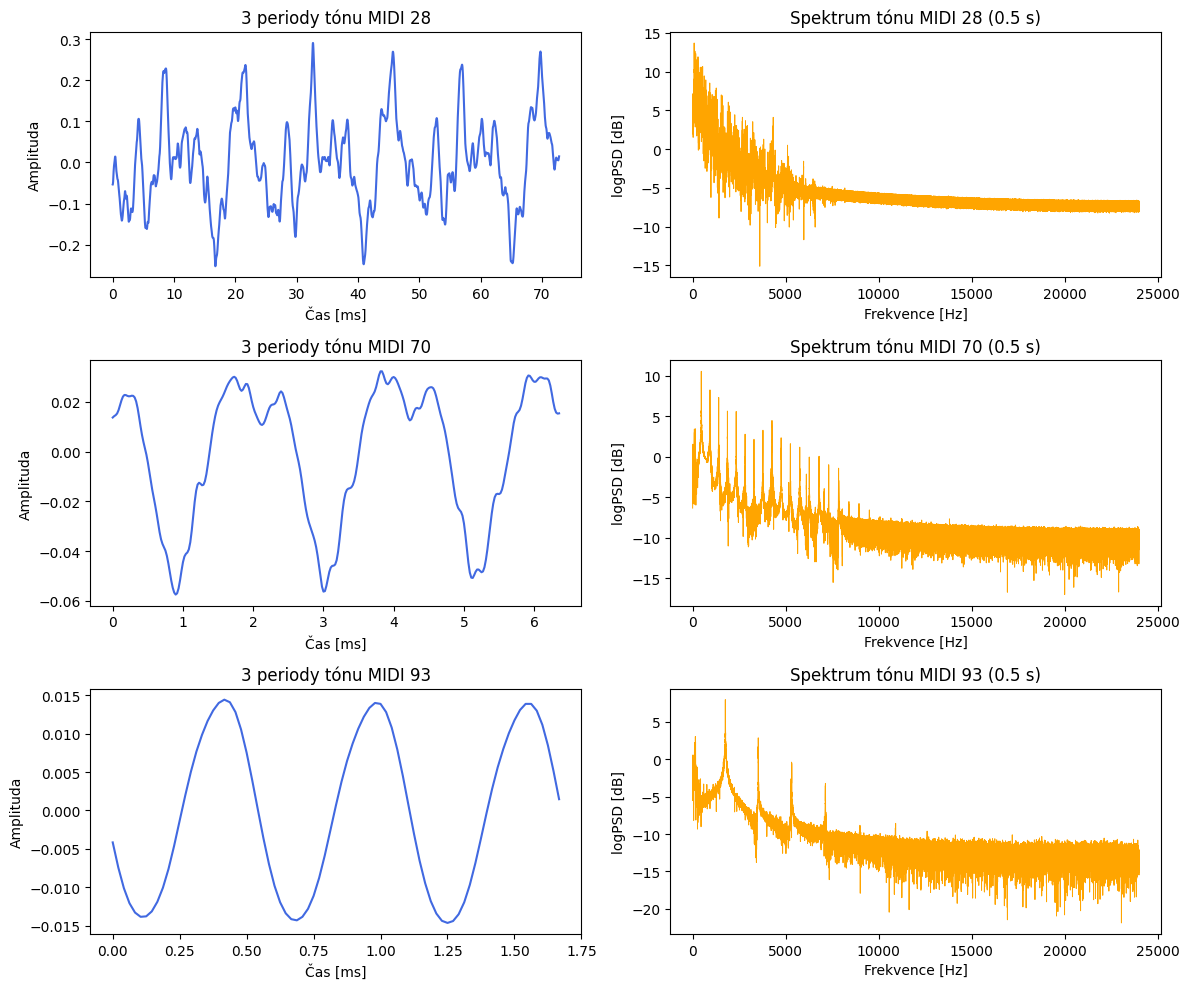
\includegraphics[width=0.96\textwidth]{out_1.png}
    \end{center}
\end{figure}

\section{Určení základní frekvence}

Pro každý tón jsem odhadl frekvenci pomocí autokorelace i DFT. 

Autokorelace byla provedena pomocí \verb|sp.signal.correlate()| a uložena její druhá polovina. Funkcí \verb|sp.signal.find_peaks()| je spočítána vzdálenost mezi největším a druhým největším vrcholem. Podílem vzorkovací frekvence a této vzdálenosti $\frac{F_s}{l}$ je spočítána frekvence. 

DFT bylo provedeno přes \verb|np.fft()|, stejně jako v 1. úkolu je provedeno doplnění nulami a uložena první polovina jeho absolutní hodnoty. Frekvence je zjištěna přes \verb|np.argmax()| z DFT.

Spočítal jsem pro obě varianty odchylku od reálné frekvence a zjistil jsem, že pro tóny do MIDI 56 je přesnější autokorelace, a pro tóny od MIDI 56 je přesnější DFT. Tyto odhadnuté frekvence jsem si uložil.

\begin{figure}[H]
    \begin{center}
        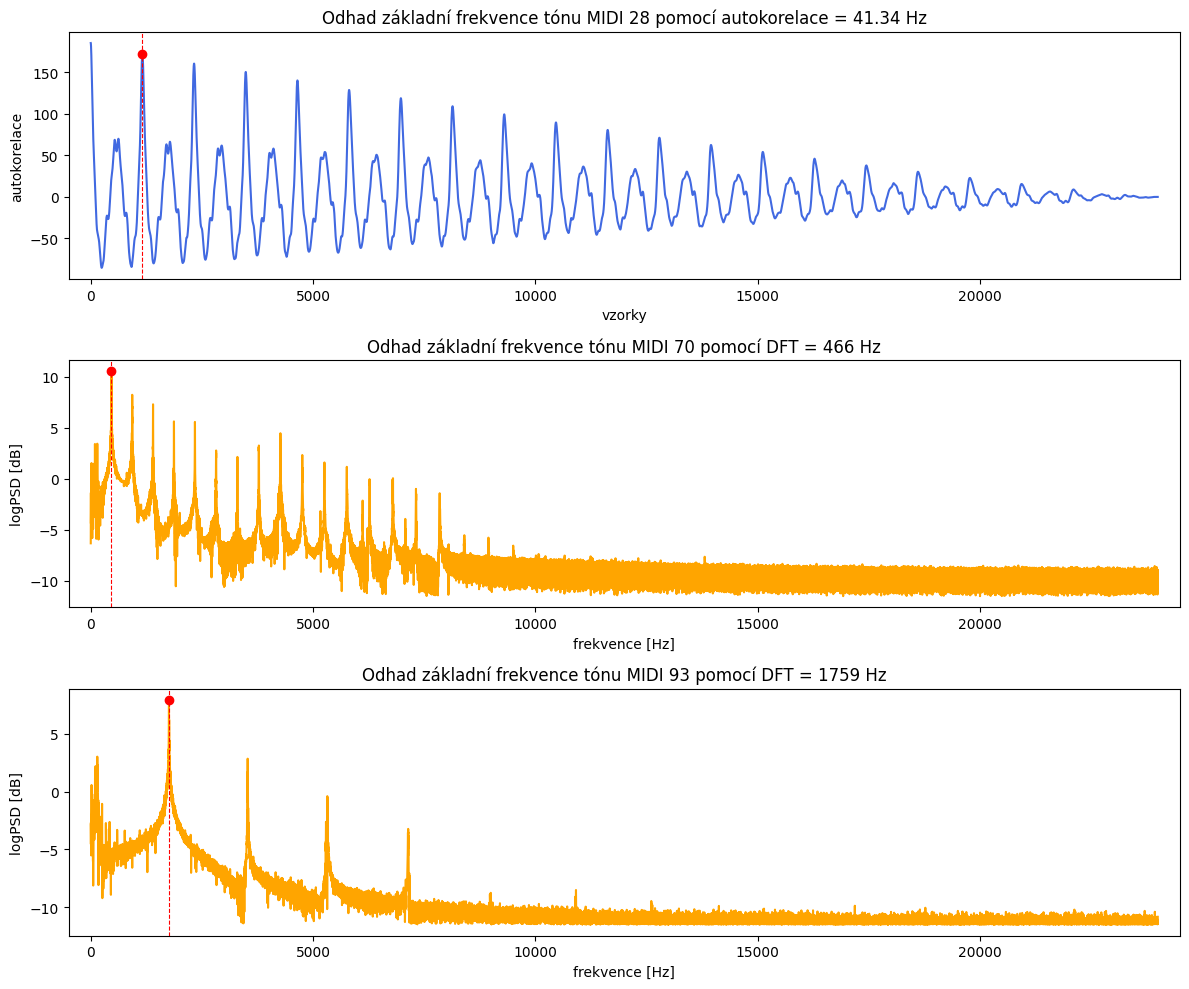
\includegraphics[width=\textwidth]{out_2.png}
    \end{center}
\end{figure}

Odchylka se u obou metod pohybuje v nižších desetinách procent, což může být způsobeno nepřesností metody, například DFT vrací pouze celá čísla, nebo přesnost autokorelace je omezena hodnotou jednoho posuvu při korelaci.

\section{Zpřesnění odhadu základní frekvence $f_0$}

Pro zpřesnění odhadu tónu je použito DTFT, kód je z velké části vypůjčen z Python notebooku k přednášce \verb|02_spectral.ipynb|. Jako hodnotu \verb|FREQPOINTS|, tedy rozlišení frekvence jsem zvolil na 500, jako optimální poměr mezi rychlostí a přesností. \verb|FREQRANGE|, tedy rozsah hledání přesnější frekvence jsem použil $1/10$ odhadnuté frekvence tónu. Na tomto rozsahu od odhadu frekvence je provedeno zpřesnění.

Pro nižší MIDI tóny je frekvence vypočítaná přes DTFT dvojnásobná, v těchto případech ukládám poloviční frekvenci.

Frekvence vypočítaná přes DTFT je zhruba ve 7 z 10 případů přesnější než odhadnutá. To, že odhad je přesnější je většinou náhoda, protože hodnota \verb|FREQPOINTS| není dostatečně vysoká.

\section{Reprezentace klavíru}

Pro reprezentaci klavíru jsem si nejprve pro všechny tóny spočítal 1- až 5-násobky základní frekvence, jenž jsem postupně pomocí DTFT obdobně jako v předchozí části zpřesňoval a další násobky přepočítal. Pro každý násobek frekvence jsem také z DTFT spočítal modul (\verb|np.max(np.abs(dtft))|)a fázi (\verb|np.angle(dtft[np.argmax(abs(dtft))]|), které jsem uložil pro další použití.

\begin{figure}[H]
    \begin{center}
        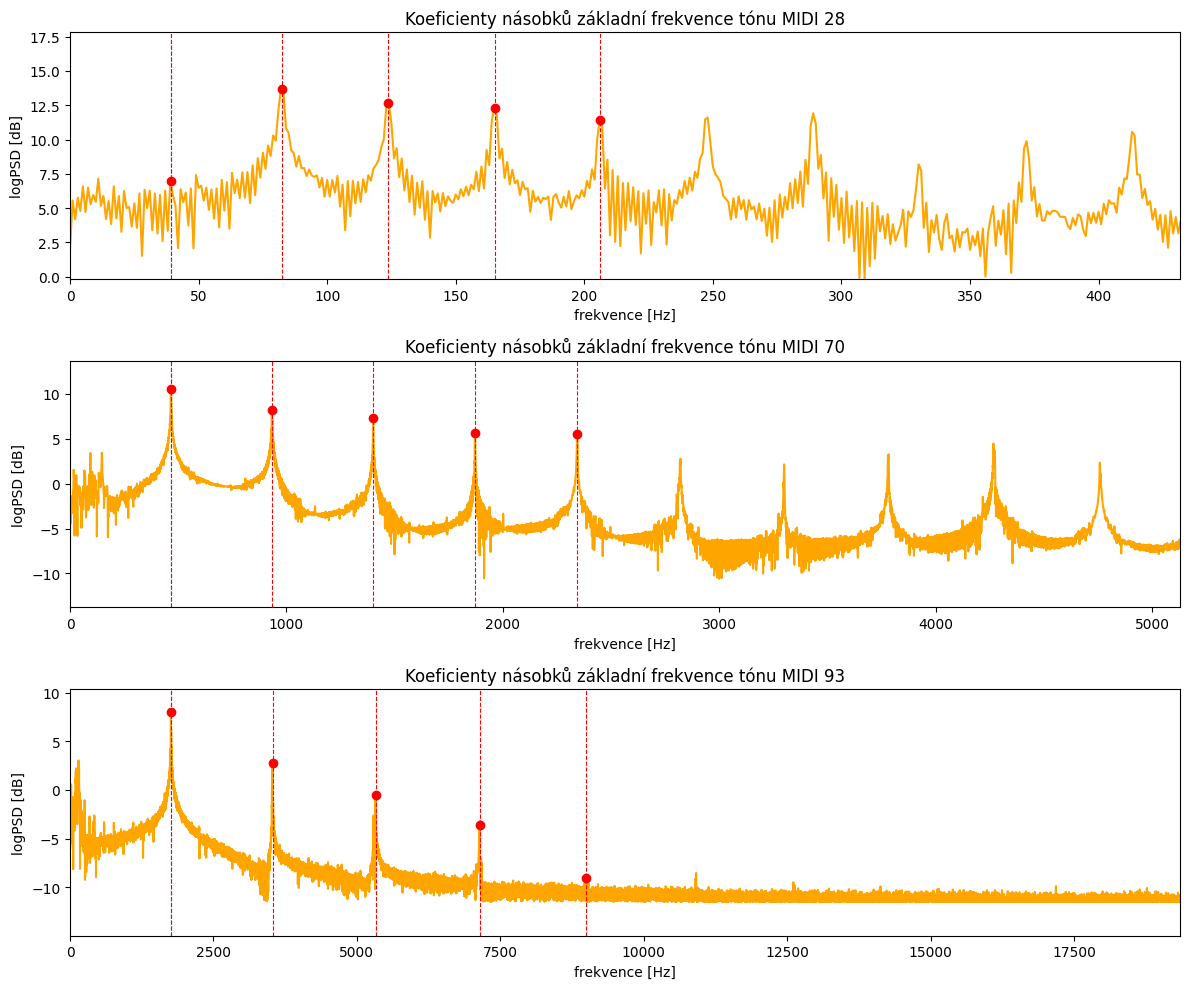
\includegraphics[width=\textwidth]{out_3.png}
    \end{center}
\end{figure}

\section{Syntéza tónů}

Syntetizování tónu provádním přes inverzní FFT funkcí \verb|np.ifft()|. Před tím, než IFFT provedu, si připravím pole o stejném tvaru (shape) jako je výstup \verb|np.fft()|, ale plné nul v komplexním tvaru. Na indexy odpovídající násobkům základní frekvence získané v minulém kroku ukládám komplexní číslo tvořené modulem v reálné části a fází v komplexní části. Modul je násoben 10, aby byl blíže původní hlasitosti.
Nad tímto polem je prováděno IFFT, z něhož ukládám 0.5 jeho reálné části.

\begin{figure}[H]
    \begin{center}
        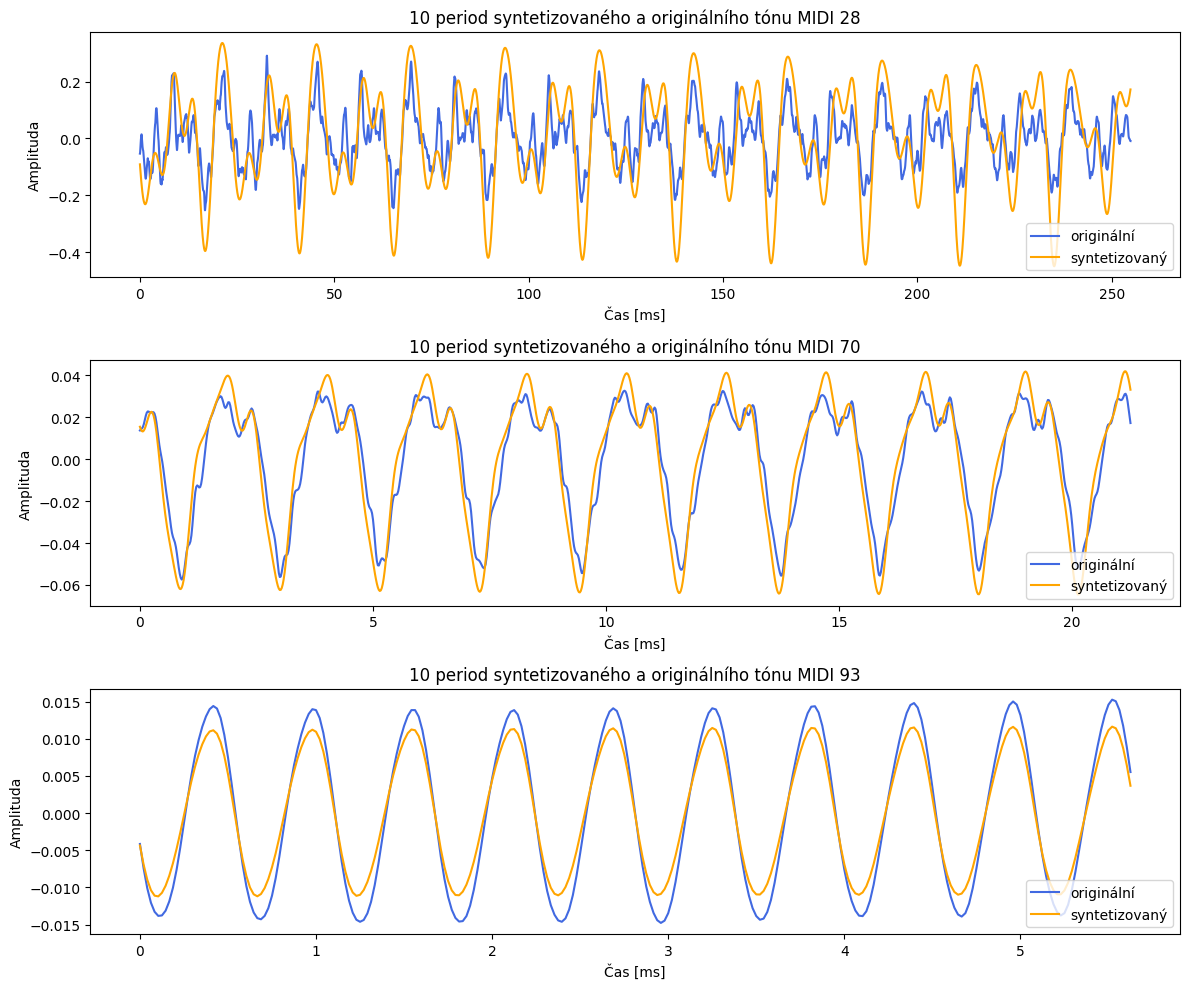
\includegraphics[width=\textwidth]{out_4.png}
    \end{center}
\end{figure}

Pro nízké tóny je amplituda syntetizovaného tónu vyšší než originálního, pro vysoké tóny naopak vyšší. Syntetizovaný tón je také hladší s méně ostrými změnami než originální, což je zapříčiněno tím, že tón reprezentujeme jen málo daty.

\newpage

\section{Generování hudby}

Data pro generování hudby jsou načítána ze souboru \verb|skladba.txt| dle zadání.

Nejprve generuji pro obě vzorkovací frekvence prázdná pole o délce skladby + 1 sekunda jako buffer, do kterých budou načítány tóny. Pro každý stisk klávesy přičítám k poli skladby tón o příslušné délce. Jelikož stisk klávesy může být delší než délka syntetizovaného tónu (0.5 sekundy), pomocí \verb|np.tile()| tón zkopíruji za sebe kolikrát je potřeba. Hodnotu hlasitosti interpretuji jako procentuální koeficient, jímž tón násobím.

Pro převod skladby o vzorkovací frekvenci 48000 Hz na vzorkovací frekvenci 8000 Hz ukládám každý 6. ($48000/8000=6$) prvek pole.

\section{Spektrogram}

Pro vykreslení spektrogramu jsem si vypůjčil kód z přednášky. Na signálu o vzorkovací frekvenci 48 000 Hz je vidět větší detail a rozlišení jednotlivých frekvencí. Na nižší vzorkovací frekvenci jsou změny ostřejší a rozdíly jsou větší.

\begin{figure}[H]
    \begin{center}
        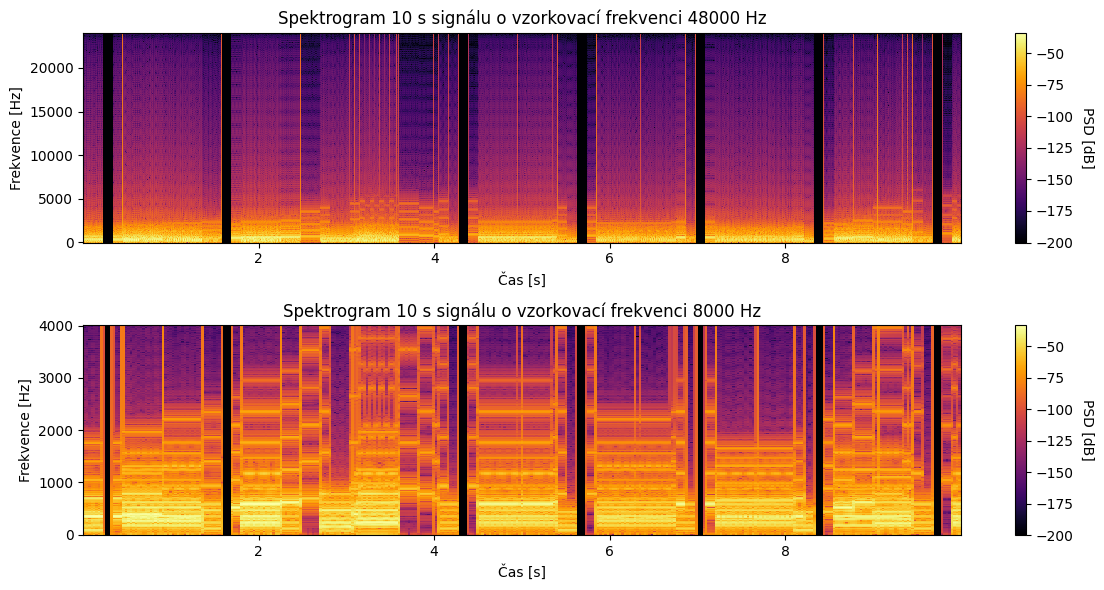
\includegraphics[width=\textwidth]{out_5.png}
    \end{center}
\end{figure}

\end{document}
